%!TEX root = ../thesis.tex
\chapter{Extraction of 3D Anatomical Structure}
\dblspace

\section{Aims} % (fold)
\label{sec:aims}
  
% section aims (end)

\section{Methods} % (fold)
\label{sec:methods}
  
% section methods (end)

\section{Results} % (fold)
\label{sec:results}
  \begin{sidewaysfigure}[htbp]
    \centering
    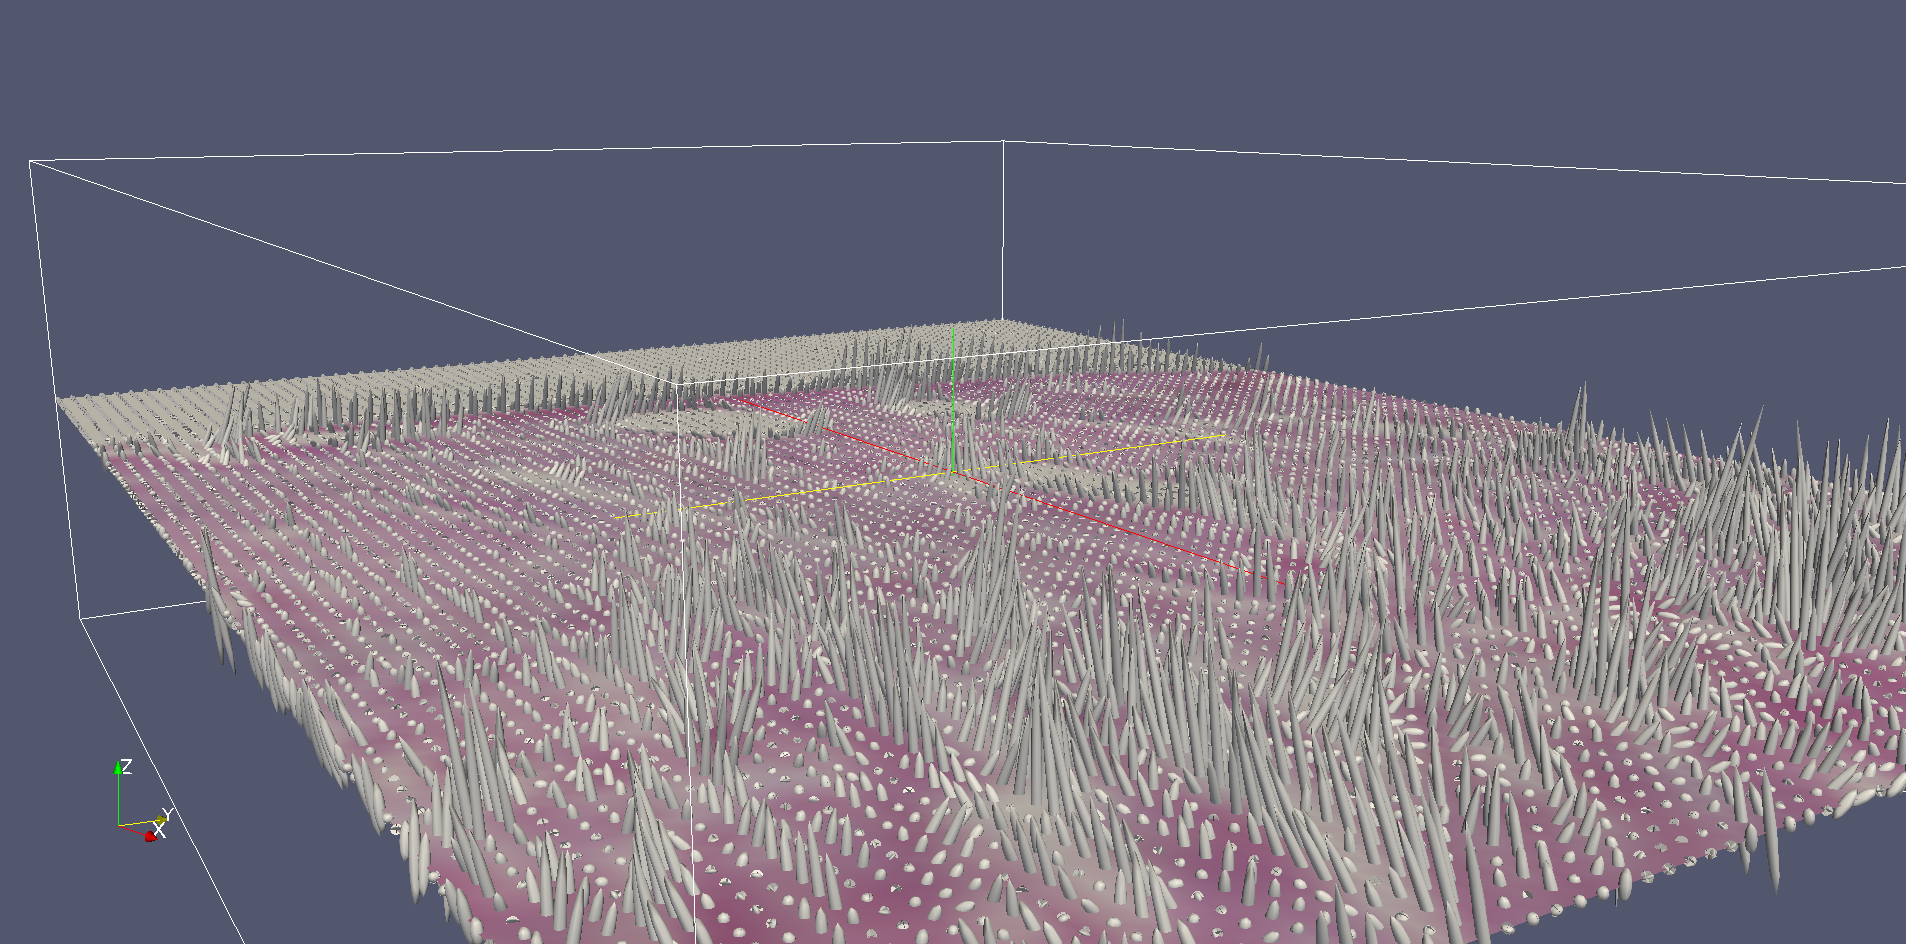
\includegraphics[width=\textwidth]{Ch8/Figs/structure_tensor_glyphs}
    \caption{A central slice through the epicardial vessel region from Section~\ref{sub:regional_diffusion}, overlayed with spheroid glyphs, scaled and oriented by the structure tensor of the pixel intensities.}
    \label{fig:structure_tensor_glyphs}
  \end{sidewaysfigure}
    
  \begin{figure}[htbp]
    \centering
    \subfigure[][x]{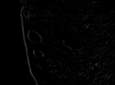
\includegraphics[width=0.45\textwidth]{Ch8/Figs/x_eigencomponent.png}}
    \subfigure[][y]{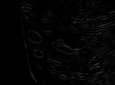
\includegraphics[width=0.45\textwidth]{Ch8/Figs/y_eigencomponent.png}}
    \subfigure[][z]{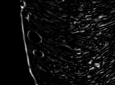
\includegraphics[width=0.45\textwidth]{Ch8/Figs/z_eigencomponent.png}}
    \subfigure[][combined]{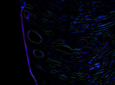
\includegraphics[width=0.45\textwidth]{Ch8/Figs/rgb_eigencomponents.png}}
    \caption{\textbf{(a)}, \textbf{(b)} and \textbf{(c)} map the absolute magnitudes of the x-, y- and z- components of the largest eigenvector of the structure tensor, of the same central slice from Figure~\ref{fig:structure_tensor_glyphs}. The volumewise maximums for the x-, y-, and z- components were 15.8, 14.6 and 68.7, respectively; the intensities have thus been scaled from 0 (black) to 68.7 (white). \textbf{(d)} combines the intensities in an RGB image, with red x, green y and blue z.}
    \label{fig:eigencomponents}
  \end{figure}
  
% section results (end)

\section{Discussion} % (fold)
\label{sec:discussion}
  
% section discussion (end)
